% %%%%%%%%%%%%%%%%%%%%%%%%%%%%%%%%%%%%%%%%%%%%%%%%%%%%%%%%%%%%%%%%%%%%%%%%%%%%%
% %%%%%%%%%%%%%%%%%%%%%%%%%%%%%%%%%%%%%%%%%%%%%%%%%%%%%%% Building on Mann 1995
% %%%%%%%%%%%%%%%%%%%%%%%%%%%%%%%%%%%%%%%%%%%%%%%%%%%%%%%%%%%%%%%%%%%%%%%%%%%%%

\chapter{Finite Poloidal Lifetimes}
  \label{ch_lifetimes}

Radoski\cite{radoski_1974} looked at \Alfven waves, using a cylindrical coordinate system to emulate an ``unwrapped'' dipole. He argued that poloidal waves should rotate to the toroidal mode over time, and that the rotation would not go the other way. 

Mann\cite{mann_1995} performed some wave-in-a-box simulations and found the rotation time to be linear in modenumber: $\tau = \frac{d \lambda}{d \omega_A'}$, where $\lambda = \frac{\azm}{2 \pi r}$ and $\omega_A'$ is the spatial derivative of the \Alfven bounce frequency. Soon afterwards\cite{mann_1997}, he supported his simulations analytically. 

Ding\cite{ding_1995} ran simulations more-or-less concurrent with Mann's. Ding saw a rotation from poloidal to toroidal... then back again. It seems that the reversal was a spatial resolution issue. 

The aforementioned models made significant simplifying assumptions in terms of geometry and boundary conditions. Neither included an ionosphere. 

Following up on this work in 3D is unlikely. Large azimuthal modenumbers are expensive to resolve, and the whole point of this result is that large modenumbers behave differently from small ones. 

%\todo{Do we see a difference between \vec{k} (momentum) and the group velocity? Poynting flux will always be pretty much along the field line, since $B_3$ is small and $E_3$ is zero, but the wave vector need not be. This is a question of coupling/converting to compressional waves, I guess. }

%\todo{Look at McKenzie and Westphal. Waves incident on the bow shock, etc, at weird angles. }

%\todo{Look at the E to B ratio. Compare to the \Alfven speed and to the height-integrated Pedersen conductivity. }

% =============================================================================
% =============================================================================
% =============================================================================
\section{Rotation of Energy}

Generally speaking, the following results are in agreement with previous results. Driving is applied to the azimuthal electric field, driving the fundamental poloidal mode. In \cref{fig_UP_UT_J_1,fig_UP_UT_J_2}, energy builds up in the poloidal fields over numerous driving cycles, then rotates from the poloidal fields to the toroidal. Simulations with large modenumber show a slower rotation. 

However, the same is not really true in \cref{fig_UP_UT_J_3,fig_UP_UT_J_4}. The driving is still applied to the fundamental poloidal mode, but there's no resonance. The driving adds energy. The resistive ionosphere sucks it out. And then the system is back where it started. It looks like a damped driven oscillator, not a resonant system. 

\begin{figure}[H]
    \centering
    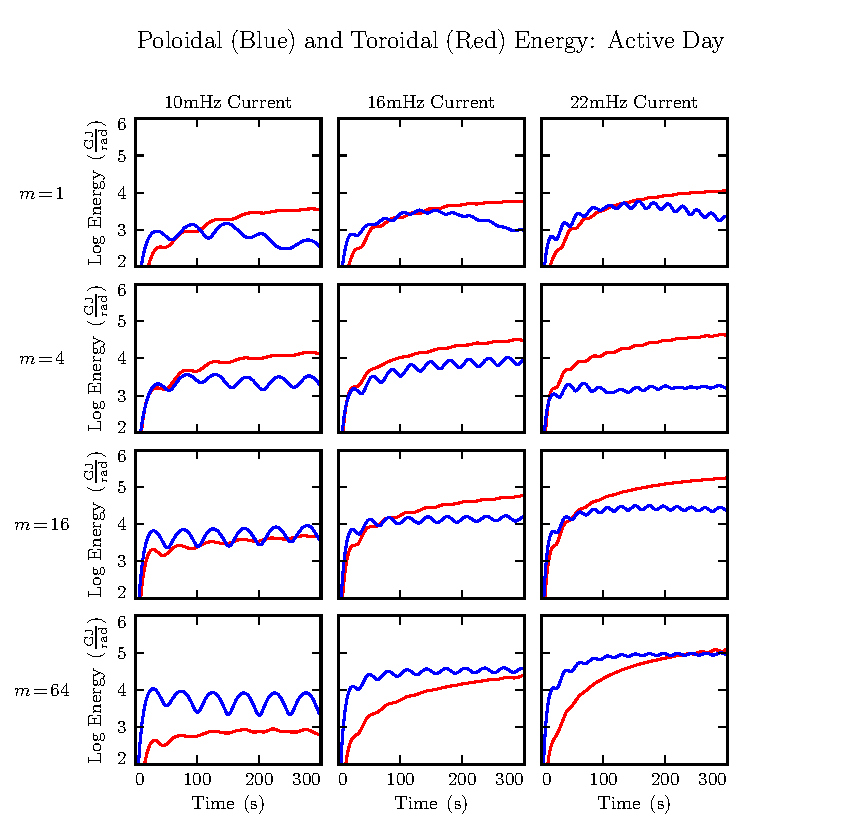
\includegraphics[width=\textwidth]{figures/UP_UT_J_1.pdf}
    \caption[Current-Driven Poloidal and Toroidal Energy: Active Day]{}
    \label{fig_UP_UT_J_1}
\end{figure}

\begin{figure}[H]
    \centering
    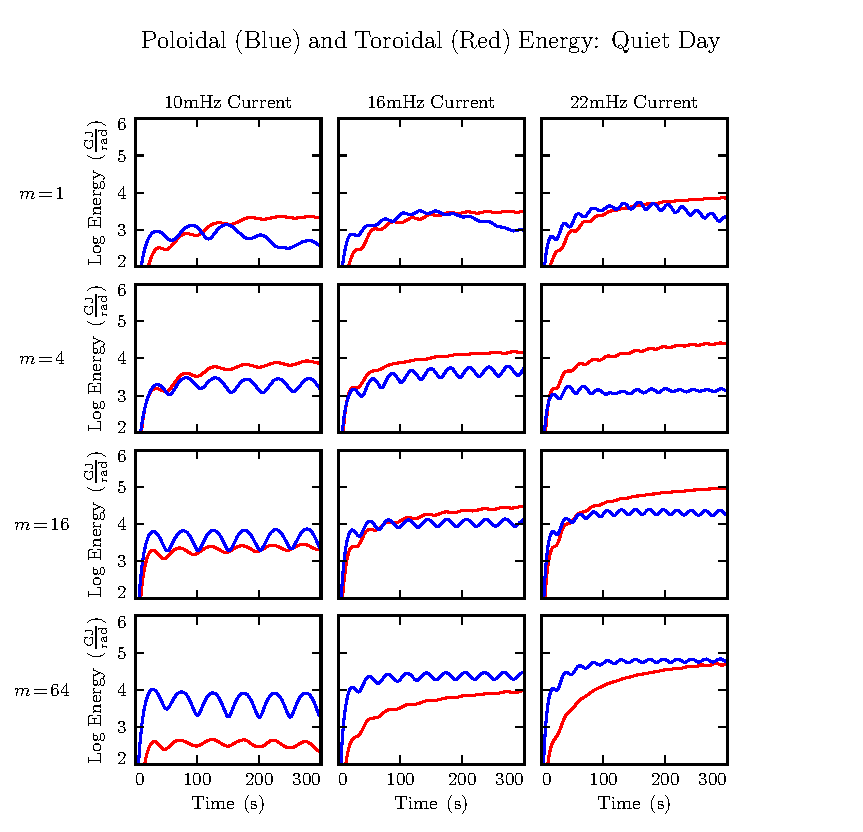
\includegraphics[width=\textwidth]{figures/UP_UT_J_2.pdf}
    \caption[Current-Driven Poloidal and Toroidal Energy: Quiet Day]{}
    \label{fig_UP_UT_J_2}
\end{figure}

\begin{figure}[H]
    \centering
    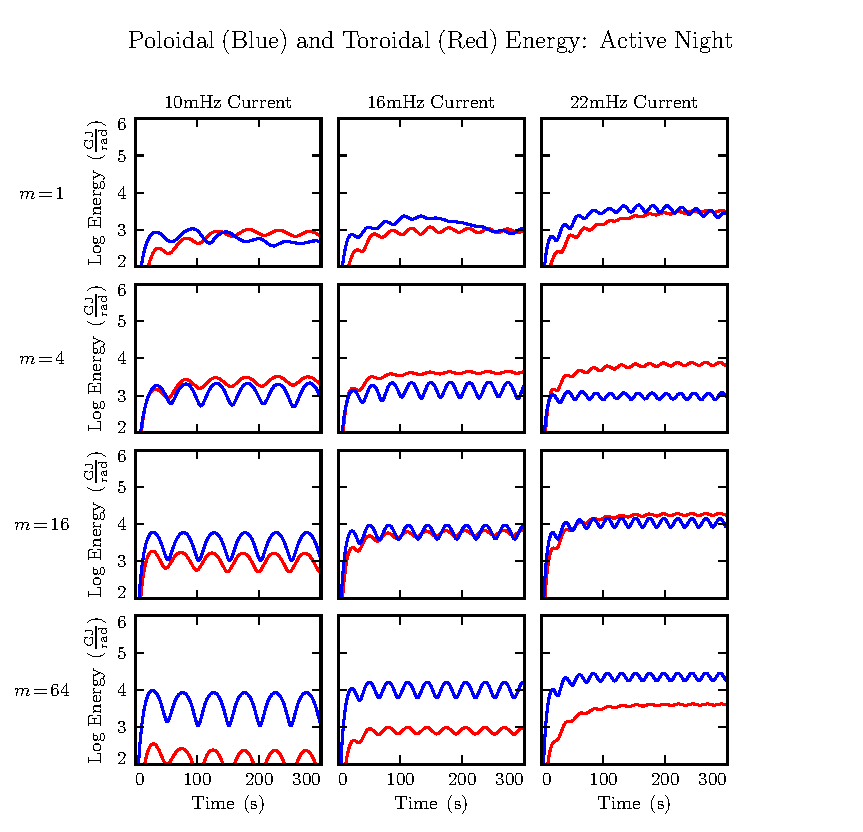
\includegraphics[width=\textwidth]{figures/UP_UT_J_3.pdf}
    \caption[Current-Driven Poloidal and Toroidal Energy: Active Night]{}
    \label{fig_UP_UT_J_3}
\end{figure}

\begin{figure}[H]
    \centering
    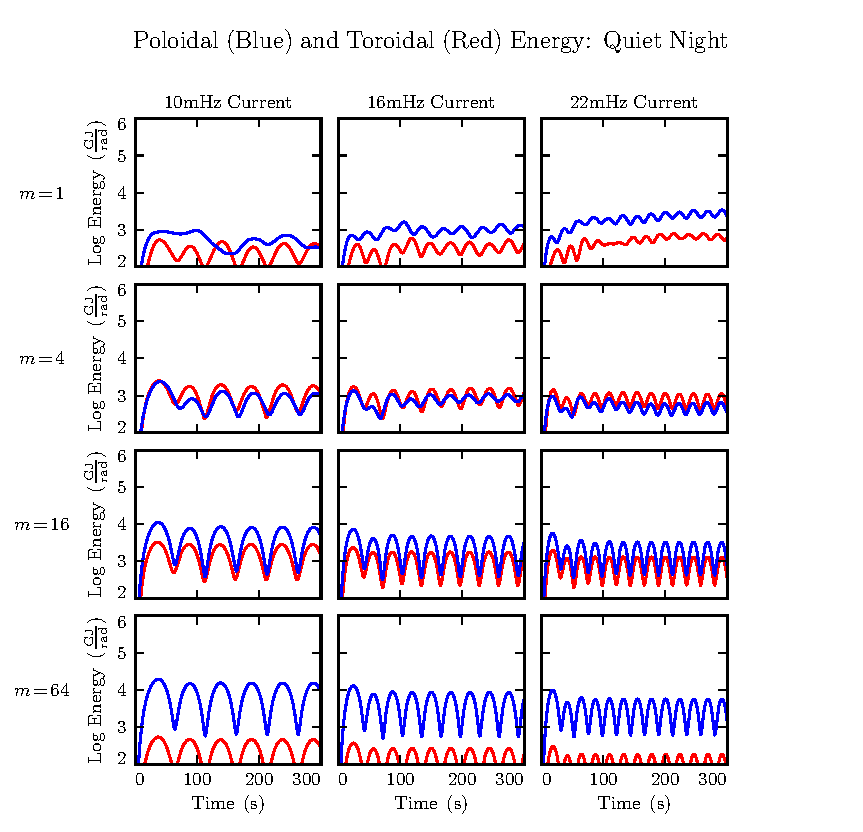
\includegraphics[width=\textwidth]{figures/UP_UT_J_4.pdf}
    \caption[Current-Driven Poloidal and Toroidal Energy: Quiet Night]{}
    \label{fig_UP_UT_J_4}
\end{figure}

% =============================================================================
% =============================================================================
% =============================================================================
\section{Resonance Feasibility}

By looking at the energy density averaged along each field line as a function of time, it's possible to get a sense for what resonates where. 

\begin{figure}[H]
    \centering
    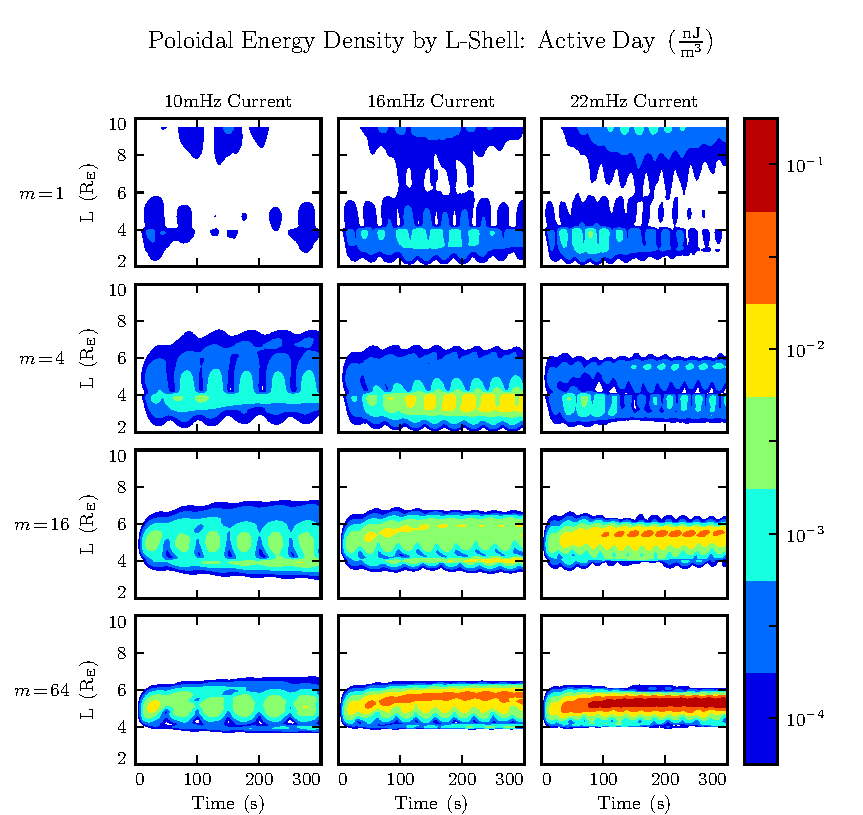
\includegraphics[width=\textwidth]{figures/upollayers_J_1.pdf}
    \caption[Poloidal Energy Density by L-Shell: Active Day]{
      In terms of structure, the poloidal mode isn't that interesting. At low \azm, it rotates to the toroidal mode too quickly to resonate; no significant amount of energy accumulates anywhere. At high \azm, the wave is guided; it never moves radially away from the location of the driving. In the rightmost column, the driving frequency matches with the resonant frequency of the driving location, so the wave resonates and accumulates energy. In the leftmost column, the driving frequency doesn't match the local bounce frequency, so nothing happens. 
    }
    \label{fig_upollayers_J_1}
\end{figure}


\begin{figure}[H]
    \centering
    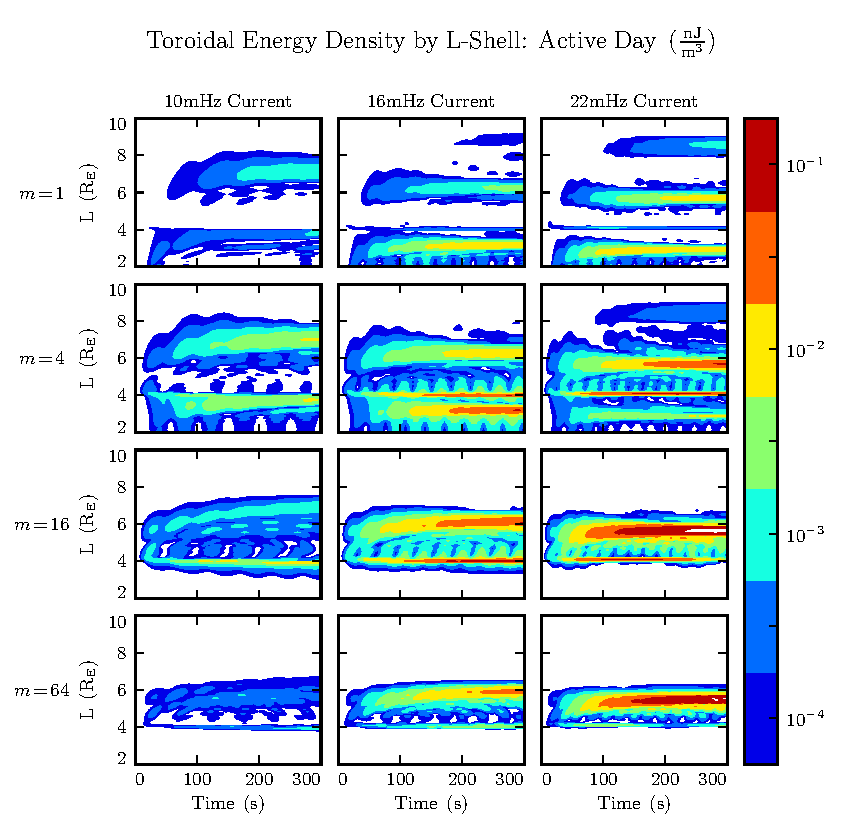
\includegraphics[width=\textwidth]{figures/utorlayers_J_1.pdf}
    \caption[Toroidal Energy Density by L-Shell: Active Day]{
      Compared to the poloidal mode, the toroidal mode has a much more interesting energy distribution. Resonances are visible both inside and outside the plasmasphere, and, particularly at low \azm, the location of wave activity is significantly affected by drive frequency. 
    }
    \label{fig_utorlayers_J_1}
\end{figure}





